 \section{Heart Modeling}
 \label{sec:heart modeling}
%The first step in any MBCT is to choose a patient model that can interact with the device in a closed loop. 
%Computer models of the heart have been developed to model different aspects of the cardiac function to suit different applications (\cite{natalia,Grosu_wave}).
%In this section we first give a brief overview of the basic Electrophysiology of the heart which describes the electrical activation and conduction, which is the basis for ICDs. 
%We also describe our effort to model the electrical activity of the heart to generate signals corresponding to a large range of heart conditions that the ICD can encounter.

\subsection{Basic cardiac electrophysiology}
\label{sec:cardiac ep}
The heart has two upper chambers called the \emph{atria} and two lower chambers called the \emph{ventricles} (see Fig. \ref{fig:icd})
The synchronized contractions of atria and ventricles assure an adequate supply of oxygenated blood to the rest of the body.
This contraction is driven by electrical activity in the heart.
A normal pattern of electrical activity is referred to as \ac{NSR}.
Disturbances of \ac{NSR} are referred to as \emph{arrhythmias}, and can result in insufficient blood supply and even death of a patient. 
\emph{\ac{VT}} is an example of an arrhythmia originating in the ventricles, in which the ventricles beat at a very high rate.
If the \ac{VT} is sustained, or degenerates into \ac{VF}, it is fatal within seconds.
An abnormally fast heart rate that originates in the atria and/or the conductinon system above the ventricles is referred to as a \emph{\ac{SVT}}.
This is not a fatal condition but does cause patient discomfort and its treatment is elective.
Many arrhythmias fall under this heading.

Implantable Cardioverter Defibrillators (ICDs) can diagnose \ac{VT} and \ac{VF} by observing the electrical activity through three channels, as shown in Fig.~\ref{fig:icd}.
The measured signals are known as \emph{electrograms}, or EGMs.
\ac{VT} and \ac{SVT} can share similar heart rates and might even occur simultaneously, so an \ac{SVT} can be mis-diagnosed as a \ac{VT}. 
This is problematic because \ac{VT} therapy consists of low and high energy electric shocks of 30-40 Joules ($\sim$800V) delivered directly to the heart, which is very painful to the patient, and has been shown to increase morbidity \cite{shock_mortality}\footnote{\small{Physicians compare a shock to a ``horse kicking you in the chest"}}.
Therefore, one of the biggest challenges for ICDs is to discriminate between \ac{VT} that typically requires a shock, and \ac{SVT} that typically should not be shocked \cite{Ellenbogen11_Pacingbook}.

An \ac{EGM} signal can be characterized by the \emph{timing of events} that produced it, and the \emph{morphology of the signal itself}.
An `event' is roughly characterized as the source of the largest peak in the \ac{EGM} (e.g. a ventricular depolarization), and event timing is a crucial element of an arrhythmia's definition in clinical Electrophysiology.
The `morphology' refers to the shape of the \ac{EGM} (see Fig. \ref{fig:adjudication} for examples).
Both aspects are used by the ICD to make its decision.
Correspondingly, our model has two components: a timing model, and a morphology model.

\subsection{Timing Model}
\begin{figure}[t]
	\centering
	\vspace{-10pt}
	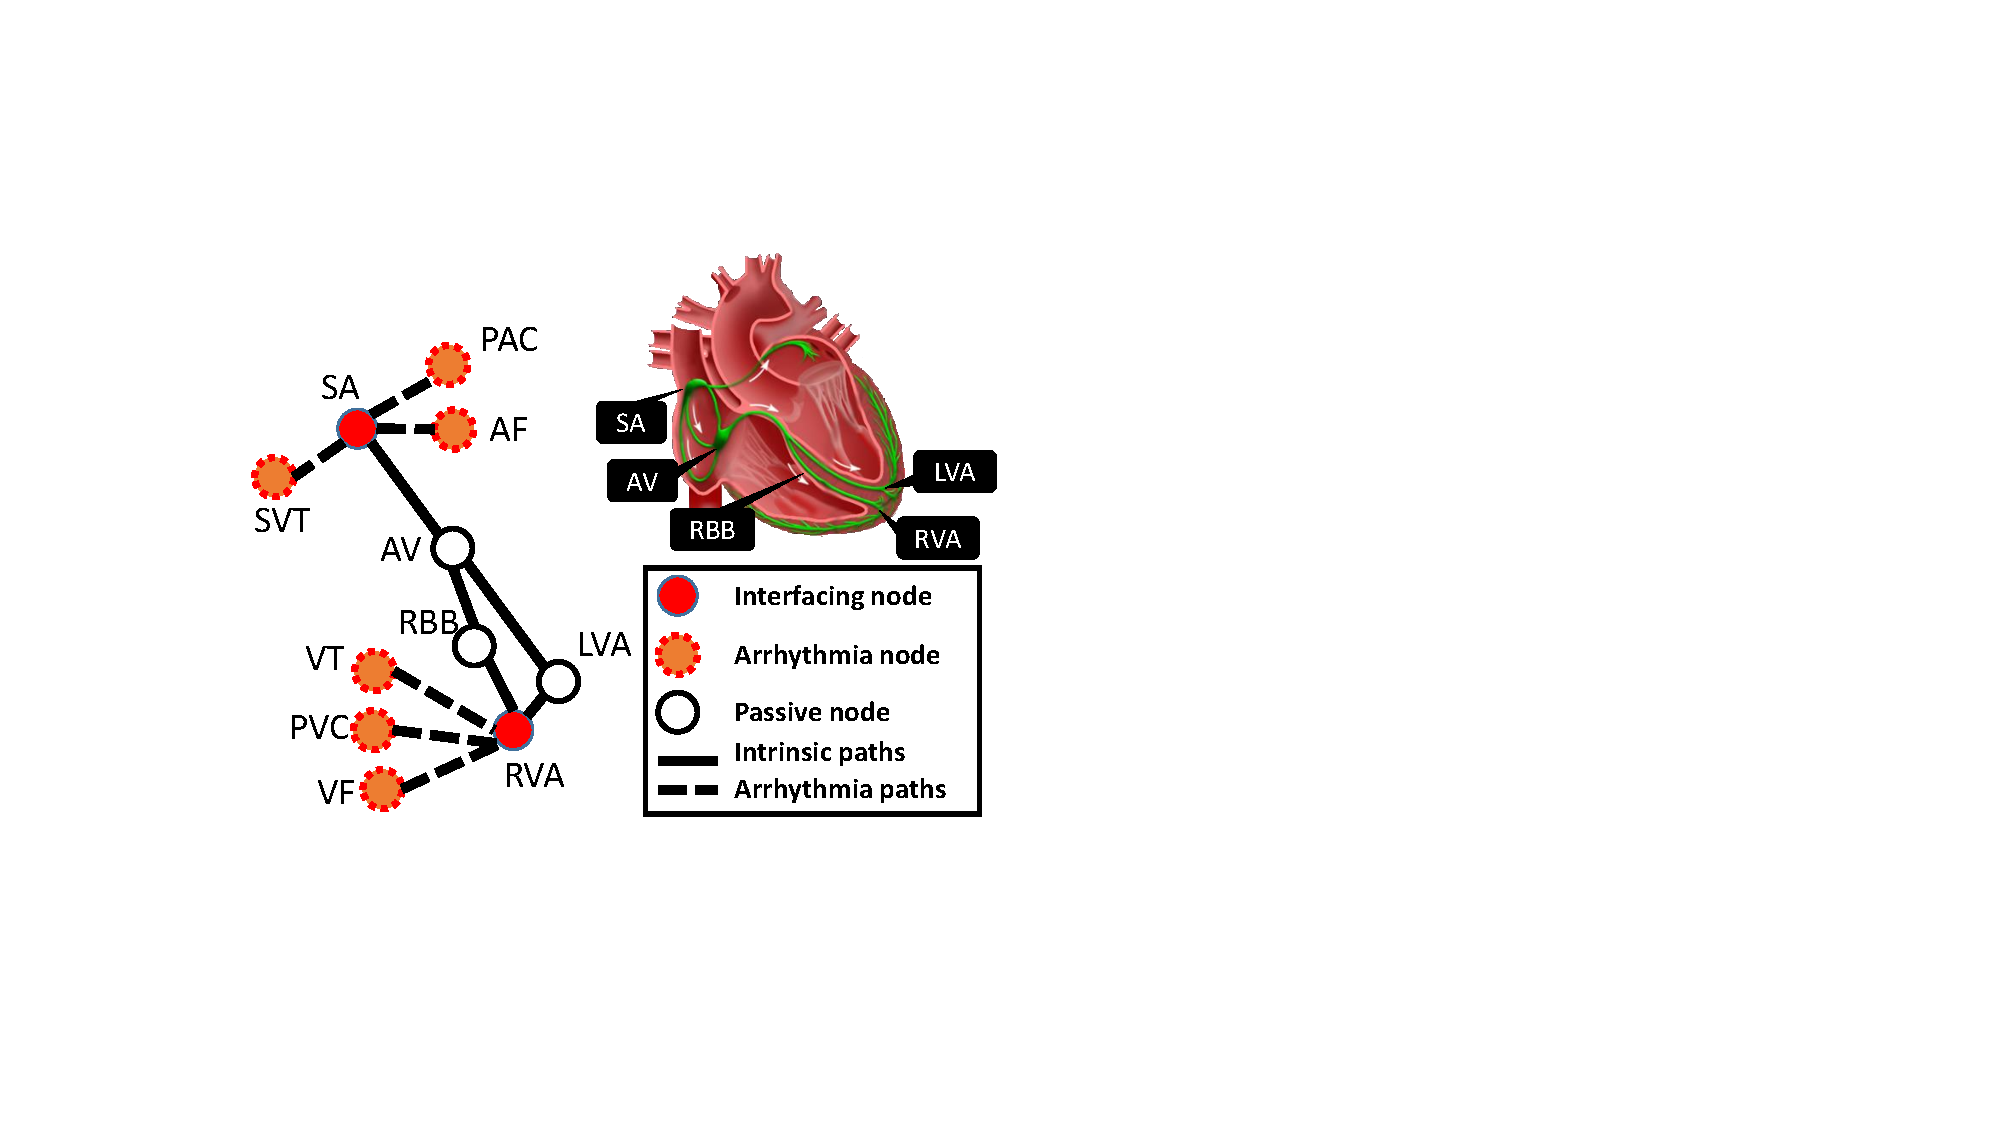
\includegraphics[width=0.3\textwidth]{figs/HM_top.pdf}
	\caption{\small Timing model of the heart}
	\vspace{-10pt}
	\label{fig:HM_top}
\end{figure}
Computer models of the heart have been developed to model different aspects of the cardiac function to suit different applications (\cite{natalia}).
In \cite{VHM_proc}, the authors developed a heart model structure that can be used to simulate the timing for generation and conduction of electrical events of the heart under a variety of conditions.
The model structure consists of a set of node automata, which model the \emph{generation} and \emph{blocking} of electrical events by heart tissue, and a set of path automata, which model the \emph{conduction delay} of electrical activity between node automata.
The node and path topology used in the \ac{MBCT} is shown in Fig. \ref{fig:HM_top}. 
The hollow nodes are passive nodes representing key locations within the heart where electrical events may be blocked. These include the Atrioventricular node (AV), Right Bundle Branch (RBB) and Left Ventricle Apex (LVA). 
The filled nodes in red, Sinoatrial (SA) node and Right Ventricle Apex (RVA) node, represent the heart locations where ICD electrodes are placed to measure the \ac{EGM}s.
The timing of the activation events at these nodes determines the timing of corresponding \ac{EGM}s.
Different sources for tachyarrhythmias are represented by arrhythmia nodes (dashed filled nodes) which are capable of self-activating at prescribed rates. These include Premature Atrial Complexes (PACs) and Premature Ventricular Complexes (PVCs) which are sources of rhythm disturbances.

Every node and path automaton has timing parameters that determine, for example, the delay between events, and how long it takes to conduct an electrical event between two nodes.
These timing parameters can be directly derived from clinical data \cite{josephson}, and the model structure is compatible with clinical Electrophysiology concepts.
Thus we know the ranges for these parameters.
In \cite{VHM_proc}, the timing model's capability to simulate various normal and abnormal heart conditions was validated quantitatively and by cardiac electrophysiologists.


In this work we use the same heart model structure to ensure the correct timing of the \ac{EGM} signals into the ICD.
%The nodes in orange are capable of self-activation at different rate determined by corresponding parameters, which represent different sources for tachy-arrhythmia.
%Since in this study we do not need the heart models to react to device therapy.
In order to account for inherent timing variability, during simulation the heart model randomly selects timing parameters within a pre-specified range, instead of choosing specific values. 
By choosing the range, we control the variability of the signals produced by a given model instance.

\subsection{Morphology Model}
The ICD uses the \ac{EGM} morphology in two ways:
first, the atrial and ventricular EGMs are used to \emph{sense} when events occur via peak detection (Section \ref{sec:sensing}).
Second, the Shock channel EGM is used in the morphology comparison discriminators (Section \ref{sec:svtvt}, \cite{VTC,Wavelet}).
It is known that sensing (the detection of events) can be responsible for up to 20\% of inappropriate therapies \cite{wrong_sensing}.
Therefore, it is important that our model generate realistic and varied \ac{EGM} waveforms for a proper evaluation of the detection algorithms.

\begin{figure}[t]
	\centering
%	\vspace{-5pt}
	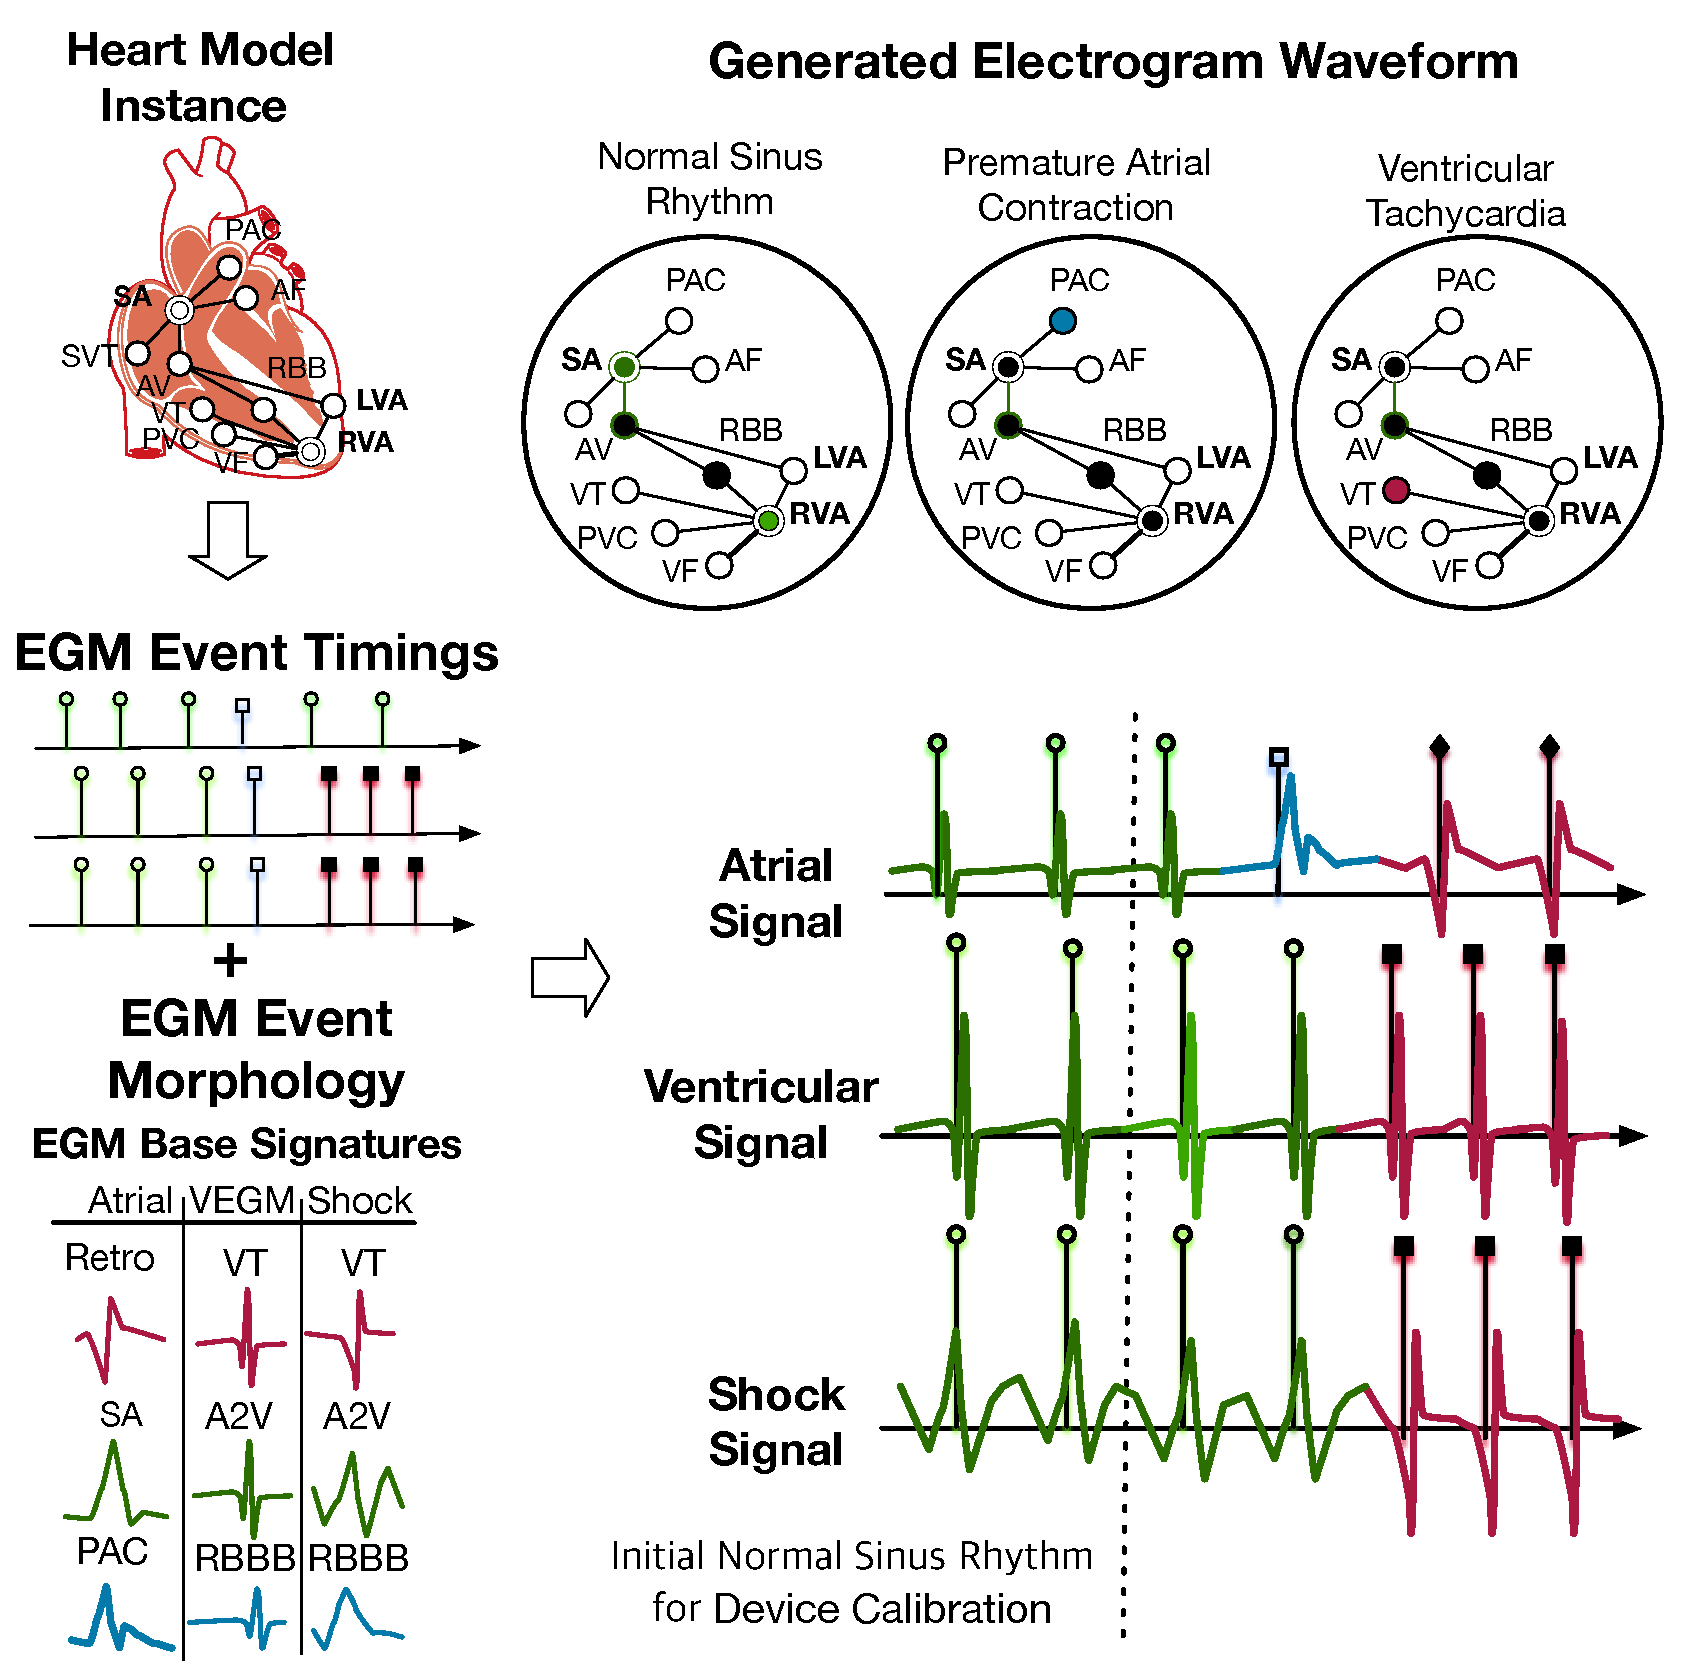
\includegraphics[scale=0.3]{figures/figEGMGeneration1column.pdf}
	\vspace{-15pt}
	\caption{\small \ac{EGM} waveform generation.
		From a given model instance and set of tachycardias, an EGM waveform is generated for the duration of an episode. The timing model determines event timings. When an event occurs, the EGM morphology for the event is output from the morphology model.  
		}
	\vspace{-15pt}
	\label{fig:egmGeneration}
\end{figure}
The timing model provides the time stamps for electrical events to happen at the interfacing nodes (SA,RVA). 
From path conduction we also know the source of the signals.
In the heart model structure shown in Fig. \ref{fig:HM_top} there are 5 different sources for SA node activation and 5 different sources for RVA node activation. 
Based on the clinical observations that electrical events from the same source produce very similar \ac{EGM} morphologies, we can generate EGM signals by overlaying EGM templates corresponding to different sources onto the timing event diagram.
The procedure is shown in Fig. \ref{fig:egmGeneration}.
We also introduce small variations on EGM templates.
The variations are obtained by a wavelet decomposition of the signatures followed by a random scaling of the 25\% smallest coefficients.
\todo[inline]{slight re-wording of preceding sentence}
We guarantee that this does not change the signature of the \ac{EGM}, by running one of the morphology comparison discriminators described in Section \ref{sec:svtvt}.
This variation is parametrized, e.g. the percentage of modified coefficients, the range of the random scaling.

 \subsection{Patient Data Adjudication and EGM Template Extraction}
In order to obtain realistic morphologies for our simulations we utilize the Ann Arbor Electrogram Libraries (AAEL), a database of over 500 \ac{EGM} recordings made during clinical electrophysiology studies~\cite{AAEL}. 
The AAEL is used by all major \ac{ICD} manufacturers and is licensed by the US FDA. 
The AAEL provides descriptive annotations of records at a high level.
We performed additional detailed examination to precisely segment each record according to rhythm type.
123 records from 47 patients were manually examined and adjudicated into segments called \emph{episodes} containing one specific rhythm, e.g.\, \ac{NSR} or \ac{VF}. 
The adjudication was performed by a cardiologist.
Fig. \ref{fig:adjudication} (left) shows an example record (Record A185660) which has undergone this adjudication.
%It should be noted that only with a standard 12-lead \ac{ECG} in addition to ICD signals can all types of arrhythmia be accurately diagnosed.
From each episode, we developed an automated process which extracted \ac{EGM}s from a given episode. 
The \ac{EGM} are collected and organized by both patient record and by the type of rhythm which was annotated during the adjudication process.
These extracted rhythm \emph{signatures} provide the basis for the morphology information in the signal generated by our model.
Fig. \ref{fig:adjudication} (right) depicts an example of 10 signatures extracted from the record. 

\begin{figure*}[t]
	\centering
	\vspace{-10pt}
	\includegraphics[scale=0.35]{figures/figadjudication.pdf}
	\vspace{-10pt}
	\caption{\small  (Left) The \ac{EGM} record is segmented into episodes with distinct rhythms in each. (Right) From each episode, individual \acp{EGM} morphologies are extracted and stored.
	}
	\label{fig:adjudication}
\end{figure*}
%(Left) Adjudication of record A185660 
%(right) Examples of \ac{EGM} morphology signatures extracted from record: SA - Sinoatrial Node Event; Retrograde - Atrial event from Ventricular Retrograde; A2V - Sinus Atrial to Ventricular Conduction; A2V Shock - Shock signal of Sinus Atrial to Ventricular Conduction; PVC - Premature Ventricular Contraction Event; PVC Shock - Shock signal of Premature Ventricular Contraction Event; VT - \ac{VT} event; VT Shock - Shock signal of \ac{VT} event;  VF - \ac{VF} event; VF Shock - Shock signal of \ac{VF} event
%Our starting point is the AAEL database of \ac{EGM}s \cite{AAEL}.
%These are \ac{EGM} records collected from real patients during electrophysiologic testing.
%We worked with 123 records from 47 patients (a patient may have more than one recording session).
%We segmented each record into \emph{episodes}: an episode is a segment of a record with one main rhythm, e.g., Normal Sinus Rhythm or Ventricular Fibrillation.
%For a given rhythm, the database generally contains several episodes.
%Then from each episode of each rhythm, we extracted a number of electrograms, say, 10.
%The extracted \ac{EGM}s provide a \emph{signature} for what the \ac{EGM} looks like during that particular rhythm.
%Fig. \ref{fig:adjudication} illustrates the process of obtaining these signatures, as well as the extracted \ac{EGM}s and the rhythms of the episodes from which they were extracted.\begin{figure*}[t]
%		\centering
%		\includegraphics[scale=0.4]{figures/figadjudication.pdf}
%		\caption{\small Examples of \ac{EGM} morphology with different signatures.
%			 }
%		\label{fig:adjudication}
%\end{figure*}
\subsection{Cohort generation}
\label{sec:cohort generation}
Let $p = (p_1,\ldots,p_n) \in \Re^n$ be the vector of timing and morphological parameters of the heart model.
Let $P_i \subset \Re$ be the range of parameter $p_i$.
We generate a \emph{synthetic cohort} of $N$ probabilistic model instances.
To produce one of these instances, for each scalar parameter $p_i$, we randomly select a sub-interval $I_i$ of its range: $I_i \subset P_i$.
The sub-interval $I_i$ is chosen so that it fits with the tachycardia that this model instance is meant to simulate.
E.g., for modeling \ac{VT}, the rest period of the \ac{VT} node might be assigned the sub-interval $I_i = [260, 280]ms$, reflecting the firing rate in the ventricles.
%Two different instances of the same tachycardia will, in general, have different sub-intervals within $P_i$.
When a model instance is simulated, each parameter $p_i$'s value changes beat to beat by sampling it uniformly within its sub-interval $I_i$.
Thus each generated model is probabilistic to reflect inherent rhythm variability.